% Figure: Grad-CAM, 3 architectures x 5 test images
% Source   : artifact/person1/gradcam/  (repo ManifoldsTeam/WoodID, branch p1,
%            commit d39a3f6b2cc5942e1e718c0dca86e89b0d81eb4d; see SOURCE.txt)
% Checkpoints: seed-42 runs of the same registry used elsewhere in this paper
% Manifest : artifact/person1/gradcam/{gradcam_manifest.csv,
%            sample_selection.csv, gradcam_metadata.json}
%
% NOTE ON ROW LABELS. The row labels printed in the figure follow botanical
% family and therefore show Araucariaceae for Araucaria araucana. This paper
% uses the four-family scheme of docs/references/WoodID_plan.md, in which that
% species is grouped with Pinaceae. The caption below names rows by species to
% avoid the clash; the figure itself should be regenerated with four-family
% labels before submission.
\begin{figure}[!htbp]
\centering
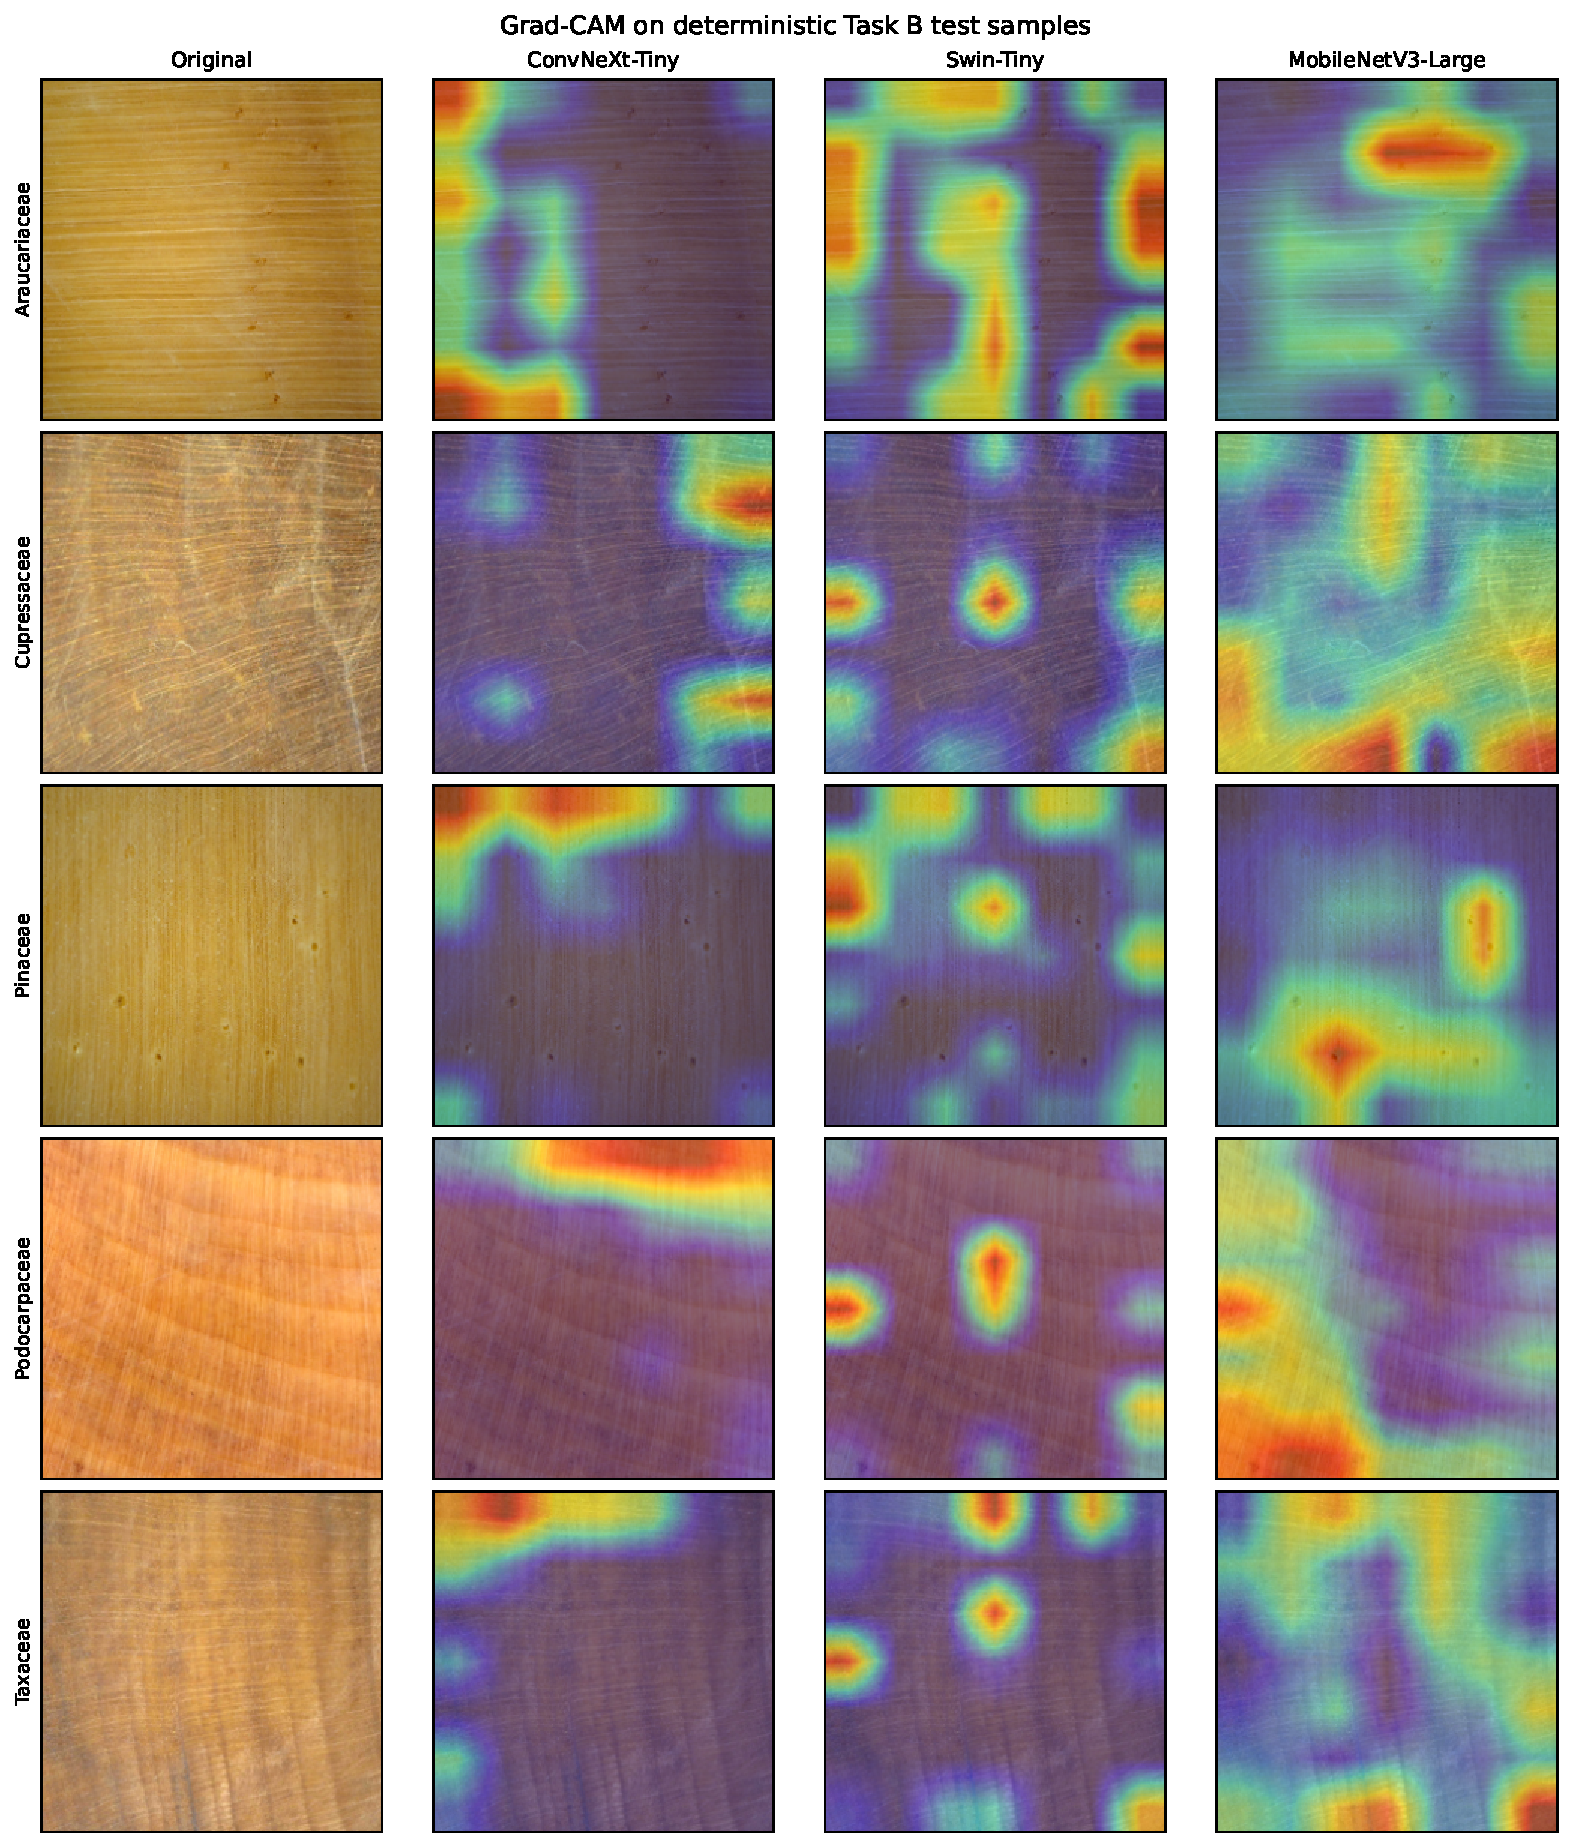
\includegraphics[width=\columnwidth]{artifact/person1/gradcam/fig_gradcam.pdf}
\caption{Grad-CAM attributions for ConvNeXt-Tiny, Swin-Tiny and
MobileNetV3-Large on five Task~B test images, one per family: \textit{Araucaria
araucana}, \textit{Calocedrus rupestris}, \textit{Pinus radiata},
\textit{Podocarpus pilgeri} and \textit{Taxus wallichiana}. Images were chosen
by a rule fixed in advance: among images classified correctly by all three
models, the one nearest the median ConvNeXt-Tiny confidence for its family,
with ties broken by image path. No image was selected for the appearance of its
heatmap. All maps come from the seed-42 checkpoints of the runs reported in
Table~\ref{tab:task_b}. Attributions are diffuse and the three architectures
highlight different regions of the same image; Grad-CAM localises gradient
support and does not by itself identify which feature is being used.}
\label{fig:gradcam}
\end{figure}
